% !TEX TS-program = pdflatex
% !TEX encoding = UTF-8 Unicode
\documentclass[11pt]{article} % use larger type; default would be 10pt
\usepackage[utf8]{inputenc} % set input encoding (not needed with XeLaTeX)

%%% PAGE DIMENSIONS
\usepackage{geometry} % to change the page dimensions
\geometry{a4paper} % or letterpaper (US) or a5paper or....

%%% PACKAGES
\usepackage{qtree} % Tree support
\usepackage{graphicx} % support the \includegraphics command and options
\usepackage{wrapfig} % Figure wrapping
% \usepackage[parfill]{parskip} % Activate to begin paragraphs with an empty line rather than an indent
\usepackage{booktabs} % for much better looking tables
\usepackage{array} % for better arrays (eg matrices) in maths
\usepackage{paralist} % very flexible & customisable lists (eg. enumerate/itemize, etc.)
\usepackage{verbatim} % adds environment for commenting out blocks of text & for better verbatim
\usepackage{subfig} % make it possible to include more than one captioned figure/table in a single float
\usepackage{url}
\usepackage{enumerate}
\usepackage{cleveref}  %cites figures intelligently
\usepackage{import} % document structuring
\usepackage{float}  %These two ensure that table position follows text by specifcing {table}[H]
\restylefloat{table}

%CODE LISTINGS
\usepackage{color}
\usepackage{listings}

\lstset{
	tabsize=4,
%	language=matlab,
        	basicstyle=\scriptsize,
%     	upquote=true,
       	aboveskip={\baselineskip},
        	columns=fixed,
        	showstringspaces=false,
        	extendedchars=true,
        	breaklines=true,
	prebreak = \raisebox{0ex}[0ex][0ex]{\ensuremath{\hookleftarrow}},
	frame=single,
        	showtabs=false,
        	showspaces=false,
        	showstringspaces=false,
        	identifierstyle=\ttfamily,
        	keywordstyle=\color[rgb]{0,0,1},
        	commentstyle=\color[rgb]{0.133,0.545,0.133},
        	stringstyle=\color[rgb]{0.627,0.126,0.941},
	language=C++
}

%%% HEADERS & FOOTERS
\usepackage{fancyhdr} % This should be set AFTER setting up the page geometry
\pagestyle{fancy} % options: empty , plain , fancy
\renewcommand{\headrulewidth}{0pt} % customise the layout...
\lhead{}\chead{}\rhead{}
\lfoot{}\cfoot{\thepage}\rfoot{}

%%% SECTION TITLE APPEARANCE
\usepackage{sectsty}
\allsectionsfont{\sffamily\mdseries\upshape} % (See the fntguide.pdf for font help)
%\ttfamily
%\sffamily\mdseries\upshape
\rmfamily
\usepackage{titlesec}
%\titleformat{\subsection}[runin]{\mdseries\bf}{\thesubsection}{1em}{}
%\titleformat{\subsubsection}[runin]{\mdseries\bf\underline\large}{\thesubsection}{1 em}{\vspace{-5 pt}}

% (This matches ConTeXt defaults)

%%% ToC (table of contents) APPEARANCE
\usepackage[nottoc,notlof,notlot]{tocbibind} % Put the bibliography in the ToC
\usepackage[titles,subfigure]{tocloft} % Alter the style of the Table of Contents
\renewcommand{\cftsecfont}{\rmfamily\mdseries\upshape}
\renewcommand{\cftsecpagefont}{\rmfamily\mdseries\upshape} % No bold!
\newcommand{\tab}{\hspace*{2em}}


%%% END Article customizations

%%% The "real" document content comes below...

\title{\Huge Motion Detection and\\Other Imaging Operations for\\Debian-Based Mobile Devices }
\date{30 August 2012}
\author{{\bf By Mehmet Tekman}\\\small MSc Computer Science\\\small University College London\\\\
\large Supervisors: Robin Hirsch and Fabrizio Pece}


\begin{document}
\maketitle 

\part*{}{\tiny.\\\\\\\\\\\\\\\\}
\begin{abstract}
Morphological image processing techniques were performed upon frames captured by the camera on the Nokia N900 smartphone to correctly detect motion for a wide variety image sizes and motion ranges using the FCam API and CImg processing library in C++ within the Qt Framework.\\\tab A commandline interface was then developed to help facilitate time lapse operations in order to efficiently watch a target within a set period of time at specified intervals. The motion detection and time lapse components were merged into a single application dubbed ‘WatchDog’ and released successfully on public repositories.\\\tab IP streaming and webcam operations were also developed but they will be implemented into WatchDog at a further date.
\\\\\let\thefootnote\relax\footnote{This report is submitted as part requirement for the MSc Computer Science degree at UCL. It is substantially the result of my own work except where explicitly indicated in the text. The report may be freely copied and distributed provided the source is explicitly acknowledged.}
\end{abstract}
\pagebreak
\tableofcontents
\begin{center}
\vspace*{\fill}
\footnote{\underline{Note:} This write up contains colors that are best viewed from the PDF file on the CD}
{\bf Acknowledgements}\\
\end{center}
I would like to thank the following people:
	\begin{description}
	\item At UCL:
		\begin{description}
		\item [Robin Hirsch] For just being all-round decent guy: very flexible with my project idea, giving perceptive suggestions, and being incredibly helpful in finding me a secondary supervisor.
		\item [Fabrizio Pece] For the speedy, concise, and friendly responses to all my queries, and for the truly helpful discussions and guidance into all aspects of the project.

		\end{description}
	\item At Home:
		\begin{description}
		\item [Family] For being notably patient and forgiving with my odd schedules and moods.
		\item [‘deed’] For being the first user on the Maemo forum to test my application upon release, and the glowing review he gave it.
		\end{description}		
	\end{description}

\pagebreak

\part{Introduction}
This project is primarily about motion detection; what it is, how it works, the various approaches attempted, and the final product. There is also a significant amount of work done on time lapse operations, and streaming over an Internet Protocal (IP Streaming).

The project was developed over the course of several months with the initial focus being about IP streaming, but later shifted attention onto motion detection as my interest in the topic grew. The time lapse was intended as an optional feature, but I found myself dedicating a week or so to it since it slotted into the motion detector code so well.
 
\begin{figure}[H]
\includegraphics[width=0.8\textwidth]{images/timeline}
\caption{Schedule and division of work}
\label{fig:timmy}
\end{figure}

{\large\bf What it is}
\begin{enumerate}
\item {\bf Motion Detector} is a device that is able to distinguish between different components of a scene (i.e. what is moving, and what is not) and react to it.
\item {\bf Time Lapse} captures images at pre-specified intervals, so that when those images are viewed successively it appears that the transition of time has increased.
\item {\bf IP Streaming} sends video or audio data from one machine to another in real time using internet protocols.
\end{enumerate}

{\large\bf What it does}
A simple example of motion detection where there is only one moving object, then often it is enough to simply subtract one image from the previous as two bitmaps and the watch the difference. The dark parts in this subtracted image would have cancelled each other out because they have not changed between frames. The parts that  ‘light up’ are parts where there was a substantial difference between one frame or the next: movement.

Rarely is there ever only one moving object in a scene, and for a scene watching a man walk past we will not want to capture the rustling trees behind him. In this case a simple subtraction would no longer work and we must perform more advanced techniques (morpholigical operations) such as eroding and/or dilating the image which shrink out or embolden features of an image respectively. Combined, they are a powerful tool and by specifying the level of eroding and dilating one can control what represents significant motion or not.
%%%HERE




\import{parts/}{background.tex}
\import{parts/}{motiondetect.tex}
\import{parts/}{timelapse.tex}
\import{parts/}{ipstreamer.tex}
\import{parts/}{userinterfaces.tex}
\import{parts/}{release.tex}

\import{parts/}{appendix.tex}

\part{Conclusions}
I believe the app has been a success. Due to the dying state of the Maemo community and the lack of N900 users it perhaps hasn’t received all the recognition that it deserves - but by itself it is a good decent application that performs a wide variety of different tasks, and does them {\it well}.

It satisfies all the requirements that a good motion detector needs such as detecting movement under a wide range of different scenarios and settings such as light/dark environments, or different types of movement such as allowing the user to specify different mask size and thresholds for large/small movement.

It even goes beyond the initial requirements and extends its abilities, such that the user can opt to have their images converted into a movie after each session, or the user can choose to be emailed for each movement that occurs (with the option to have the image containing the movement emailed to them). This gives the application new function, so that it is no longer just a motion detector, but a full-blown security device that can notify and alert its owner of activities around the phone (such as emailing the mugshot of the guilty culprit attempting to steal something of the owner’s).

The implementation of the commandline emphasizes this side of the application, since the user does not have to be within the vicinity of the phone to set up the watchdog, but can now ssh or telnet into the device remotely and perform operations without anyone knowing. This greatly extends its security applications by enabling the user to convert their phone into a spy device at will.

The time lapse operations give a sense of novelty back into the application so that the more artistic users can compile movies of objects moving over the course of days, and the native integration of the scheduling the photos using the phone’s native scheduler makes it feel less of a burden, since it does not require installing any extra dependencies.

The IP streaming part of the application shifts back towards the practicality of application, much like the motion detector, but away from the security side of things and more for use as a video conferencing tool, so that the user can be moving about anywhere and streaming it live to a remote computer elsewhere.

On Maemo, there is nothing like this app out there on the repo’s. However on other platforms, there are plenty of contendors who have more complete version of different {\it parts} of my app:

Windows mobile already has a motion detection app ‘Vio’\footnote{Vio detection - http://vio-detection.com/}\label{ref:vio} which boasts features similar to mine (email user with image, convert to video), but can also send an SMS text.  I didn’t think to do that feature myself, mostly because  I have a pay-as-you-go contract and so don’t rely on network services (most of my communication is IP-based), but the implementation is easy to do especially since the QtMobility framework simplifies these tasks. 

Vio lacks a commandline interface, and is closed-source. For me these are major contesting points, since a user should have access to their phone in every way possible, and they should also know that the security software they have just installed on their device is not itself a security risk (which is why I dont trust AVG or Avast AntiVirus software).

iPhone and Android have similar motion detectors (e.g ‘Motion Detector’ for iPhone\footnote{Motion Detector - http://itunes.apple.com/gb/app/motion-detector/id331443079?mt=8}, and ‘Motion Detector Pro’ for Android\footnote{Motion Detector Pro - http://motiondetector.homepagepublisher.com/}), both of which have plenty of downloads but are not as fully developed as my app is in terms of features.

Once the IP streaming component is well integrated into the application, I believe it will become a must-have app due to sheer multitasked functionality that it offers.

I’ve previously discussed porting the app to future phones, most likely Windows Mobile due to Qt being well-integrated into it, and this is the aim at the moment. Before I do that I need to secure a loyal fanbase who are familiar with my work, so I believe a required stepping stone for transitioning from Fremantle to Windows (without being called a traitor) is Harmattan . Due to Fremantle and Harmattan (Meego) using a similar framework, porting from one to the other will not be difficult and will help secure a loyal fanbase, since most of hardcore N900 Fremantle users switched to Harmattan N9 rather than choose the alternative (iPhone, Android, Windows).

In the meantime, the app serves as a good end product for a neglected (but otherwise fantastic) phone and may be a possible winner of the Maemo 2012 Coding Competition.

\begin{thebibliography}{9}

\bibitem{vio}
Vio Detection, Motion Detection Application,
\url{http://vio-detection.com/}

\bibitem{moip}
Senstic , Motion Detector, Iphone
\url{http://itunes.apple.com/gb/app/motion-detector/id331443079?mt=8}

\bibitem{moan}
Motion Detector Pro, Android, (Anonymous Developer)
\url{http://motiondetector.homepagepublisher.com/}

\end{thebibliography}


\end{document}

